\chapter{Discovering archetypes of behavioral evolution}
\label{chap:evolution}
In this chapter, we aim to discover archetypical patterns of behavioral evolution among users. In our work, an archetype comprises of \emph{progressive stages} of distinct research \emph{behavior}. We introduce a novel Gaussian Hidden Markov Model (G-HMM) cluster model to identify archetypes of evolutionary patterns. G-HMMs allow for: behavioral variation and different evolutionary rates; impose constraints on how individuals can evolve; and are interpretable.

We evaluate our approach to an interesting domain of patterns of change in research interests of scientists with experience. In addition, we evaluate our model for activity distribution evolution of users in StackExchange communities to showcase the generality of our framework \cite{evolution}.


\section{Overview}
\label{sec:Introduction}
In this chapter, we develop models to understand how individuals evolve with experience in social networks. The problem is important: as individuals interact with each other, they gain in experience, and behavioral changes reflect the newfound experience. However, despite a significant focus on community discovery and their evolution in social networks, our understanding of individual evolution is limited (\citet{Yang:2011, McAuley:2013} are some notable exceptions). Understanding evolutionary patterns, in general, is useful in a variety of applications: language evolution~\citep{Danescu}; expertise evolution~\citep{McAuley:2013}; journey optimization in digital advertising platforms.


Our specific interest lies in understanding how academics change their research behavior with gain in research experience. In the academic community, authors' research interests are influenced by other authors' directly (collaboration) or indirectly (related published research) and in general, by the current research trends in the community. Analyzing the evolution of academic behavior on the community level has attracted persistent interest; previous works studied the evolution of research themes for a particular scientific community \cite{Li:2011} or multiple communities \cite{Biryukov:2010, tanmoy:2013}.
On an individual level, evolutionary studies have looked at modeling career transitions \cite{Danai:2018}, citation evolution \cite{dashun:2013} and  productivity or collaboration trends \cite{Way:2017}. On the other hand, in this work, we want to identify dominant patterns of \emph{research interests} evolution common among academics across different subfields. Our work can help to answer questions like, Do academics focus on a single research area throughout their career or they venture in multiple areas as they gain experience? If they work on multiple areas, when does this shift usually happens? Are some evolutionary patterns preferred over the others? This knowledge can assist in providing better career guidance to junior faculty on how to structure their career. Moreover, it can help funding agencies identify researchers of particular evolutionary pattern that may need more assistance.


At the outset, discovering patterns of individual evolution appears to be a combinatorial problem: academics vary in not only the sub-field that they choose to start but also in subsequent areas of interest. Furthermore, their research interests may evolve at different rates. Despite variations in the chosen sub-field of an academic, and how academics can evolve, we observe regularities at different stages of their career. For instance, for an academic, transition through different stages--- Ph.D. Student (focusing on a single research area), being an assistant professor (working on few highly related areas) to eventually post-tenure (multiple areas, interests in multidisciplinary collaborations, etc.)---mark changes in research behavior. These elementary behavioral evolutionary patterns are visible in almost all academic fields, suggesting that surface variations (i.e., area of research for an academic) hide deeper regularities in patterns of behavioral change. We refer to these \textit{latent} regularities in individual behavior as \textit{behavioral stages}. We refer to the dominant progression patterns through behavioral stages as \textit{archetypes}. Note that researchers may evolve at different rates through these stages. We show that we can explain all individuals' surface variations (the observed research area on which the academic focuses) with a small set of such archetypes. ~\Cref{fig:example} shows a stylized example.

Thus a model for learning archetypes needs to: express variation in observable research behavior while exhibiting latent stochastic regularities governing the change of behavior. Furthermore, the model should allow individuals to evolve at different rates. Finally, the results ought to be interpretable in a post-hoc manner.

\begin{figure}
 \centering
  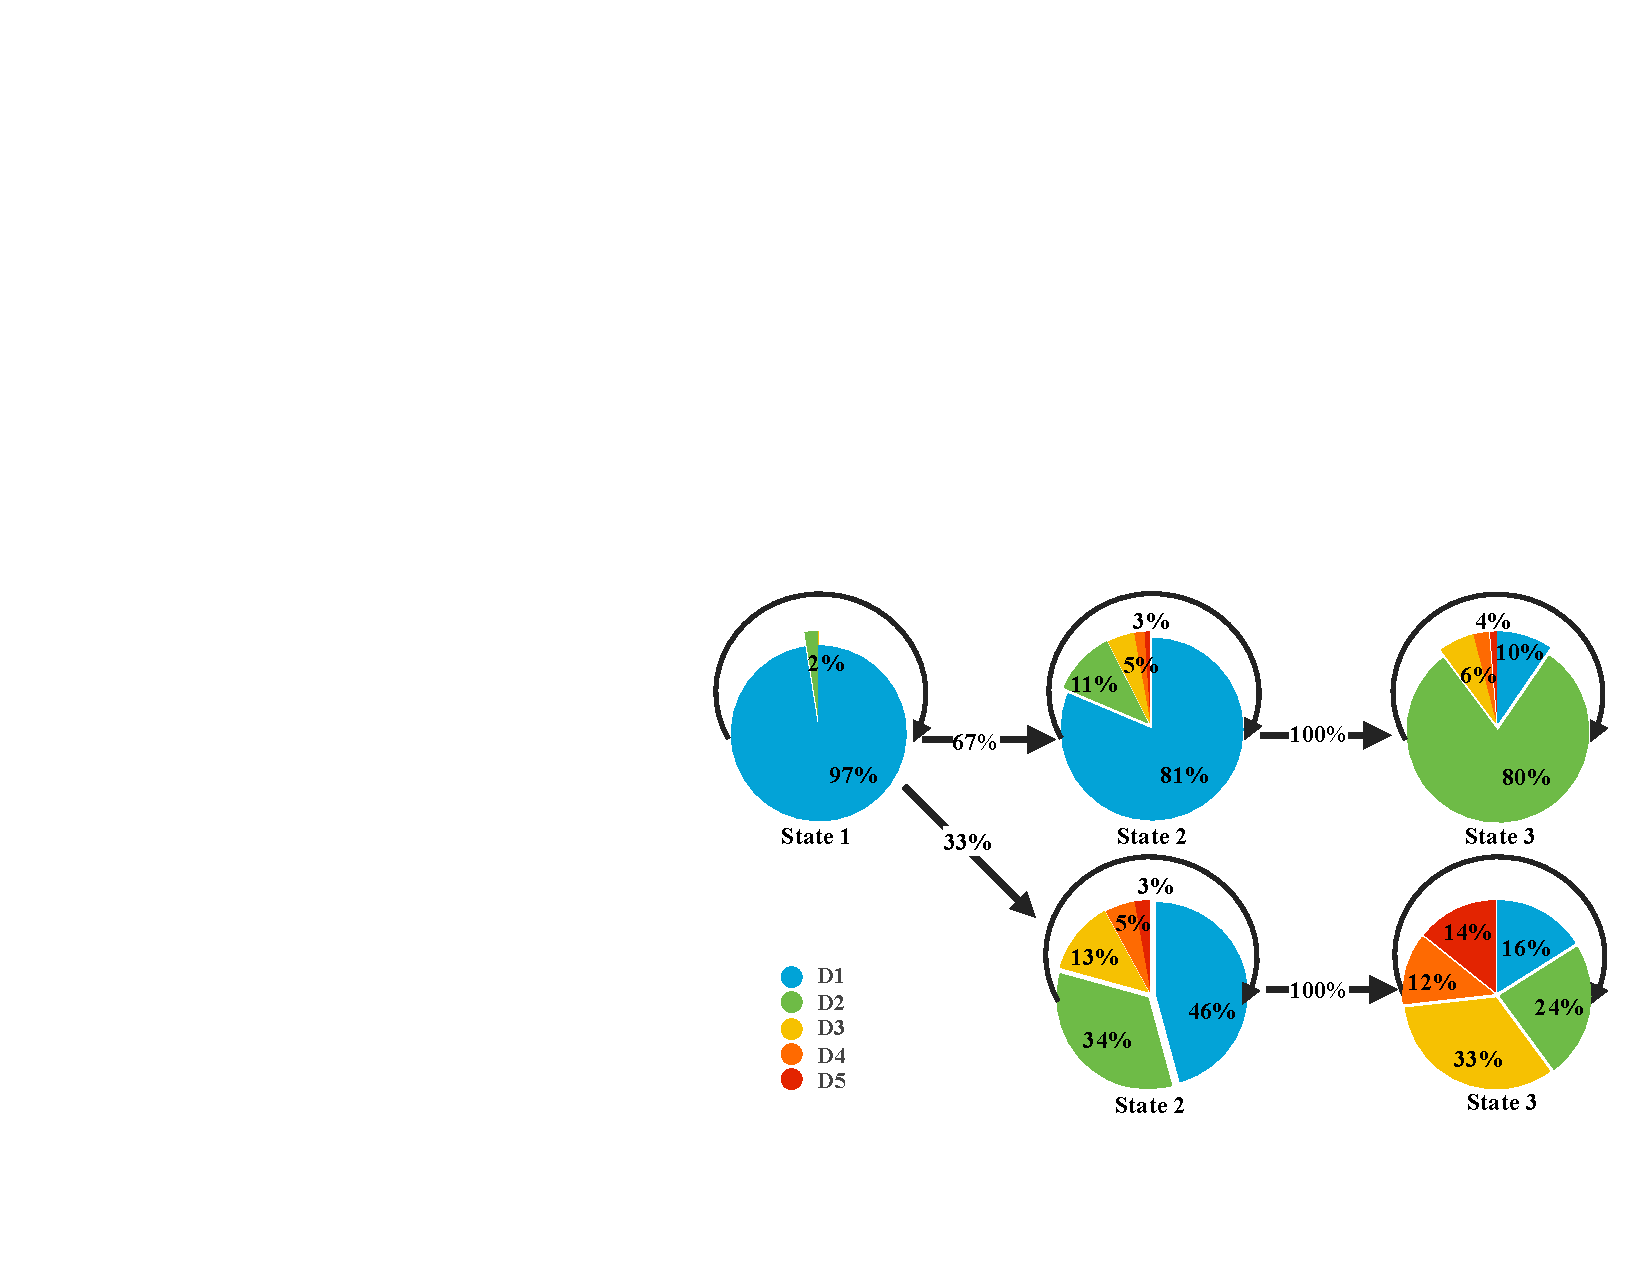
\includegraphics[width=0.7\linewidth,height=6.4cm]{figures/Example_figures_Self.pdf}
 \caption{\label{fig:example} A stylized academic evolutionary trajectory. Each pie chart is a \emph{behavior stage} in the trajectory. The numbers in each pie-chart show the fraction of chapters published in each research area \textit{$D_m$} in that stage. We use a normalized representation focused on the change of areas: the label $D_1$ represents the first research area of every academic, $D_2$ the second research area, etc. Normalized representations allow us to discover commonalities in behavioral changes of academics across seemingly unconnected domains. In this example, the top group of researchers evolves to shift their research focus to a new domain while the bottom group becomes increasingly interdisciplinary.
 }
\end{figure}

\noindent
Our work makes the following contributions:
\begin{description}
\item[A framework for modeling evolutionary trajectories:] We propose a sophisticated framework to identify dominant, interpretable, evolutionary archetypes amongst academics for modeling the evolution of their research interests. In contrast, prior work on academics has either focused on the qualitative analysis (e.g.,~\citep{Ward:2001}) or predicting career transitions~\citep{Danai:2018}. In our work, we assume that an archetype is a \emph{probabilistic model} that encodes individual progression through stages of \emph{distinct} behavior. Specifically, we learn a Gaussian Hidden Markov Model (G-HMM) to capture this progression where latent states capture \emph{behavioral stages} in the evolution. To encode the idea of experience, while we allow individuals to evolve into the higher stages, we constrain our model to prevent individuals from returning to a stage from which they have evolved. We model \emph{all} individuals with a \emph{small} set of archetypes. We jointly learn the mapping of users into their archetype and the archetype's associated model's parameters through an Expectation-Maximization framework.
\item[Finding: Dominant archetypes:] While our framework is generic, we apply our model to understand the evolution of the research interests of Computer Scientists. We identify four archetypes with almost equal distribution of academics: (i) \emph{Steady} researchers who primarily work in their first research area throughout their career (most popular); (ii) \emph{Evolving} researchers, who continuously shift their dominant area of research; (iii) researchers with \emph{Diverse} research interests; and (iv) researchers who have \emph{Diffused} interests with infrequent contributions in multiple areas. Each archetype is significantly different ($p< .001$) from the others.
\item[Finding: variation by gender within archetype:] We examine empirically, a subset of our data---all full professors (as of Spring 2018) in the top 50 CS departments in the United States for gender differences in their academic trajectory. We observe similar gender distribution across archetypes with the least number of women professors in \emph{Evolving} archetypes.
However, within the same archetype, we observe significant differences in the models that explain the evolution of male and female researchers. For instance, the models that explain women and men differ ($p< .01$) in the \emph{diverse} archetype; we observe 30\% men (8\% women) tend to start from later stages while women skip more stages (50\% women (36\% men) skip stage 3; 14\% (9 \% men) women skip stage 2). Women also spend around a year more \emph{exploring} mid-career than men (6.5 years for women vs 5.3 years for men) in the same stage.
\item[ Finding: variation in grant income:]  Next, we examine grant income (as of Spring 2018) from the National Science Foundation in the US for the same subset of CS academics, to understand the relationship between variations in awarded grant income over the course of academic trajectory and how difference in archetype or gender could serve as explanations.
Although we did not observe any significant changes in the average grant income between archetypes, there exists income variability within stages of each archetype.
In general, researchers are awarded more grant money as they gain experience, with the most notable uptick being after the first few years of their research career (between stages 2 and 3, $p< .001$) and in their last career stage (stage 5, $p< .05$).
Specifically, researchers with \emph{diverse} research interests receive subsequently increasing grant income while \emph{evolving} researchers (who change their dominant research area in each stage) experience grant income variability with an area change.
We find significant differences in grant income across genders \textit{within a behavioral stage} of an archetype also mostly accompanied by an area shift. For the \textit{steady} and \textit{diverse} archetype, female professors are awarded lower grant income than their male counterparts ($p< .05$) in their early career stages. On the other hand, evolving women receive a significantly lower income than evolving men when they switch to new areas later in their career in state 4 and 5 ($p < .05$).
\end{description}

Also, we have strong quantitative results with competing baselines for behavior prediction and perplexity on the Academic dataset.
We subsequently evaluate our model to multiple StackExchange communities to show generality of our work.
The proposed G-HMM cluster model improves by 24\% for Academic and on an average of 32\% for Stack Exchange communities over the baselines for behavior prediction.
Our model also exhibits lower perplexity than the baselines.

\textbf{Significance:} We propose a sophisticated probabilistic framework to identify dominant, interpretable, evolutionary archetypes. We show that the discovered archetypes are significantly different and are straightforward to use to test hypotheses (e.g., evolutionary variation with gender; effects of gender on income). 
